\documentclass[../main.tex]{subfiles}

\begin{document}

\problem{3}

One-dimensional, steady, compressible flow is used for a number of real-world applications, including: normal shock waves, bow shock waves, etc.
Look up some images or videos of normal shock waves and bow shock waves in front of bullets, re-rentry vehicles, etc. 
A schematic illustrating such flow is given below, where the flow entering the dashed control volume is given as state 1 and the flow exiting as state 2.
We will learn later in the semester that these properties do indeed change across shock waves.
For now, we will focus on simplifying our governing equations for these assumptions. 

\begin{figure}[ht]
    \centering
    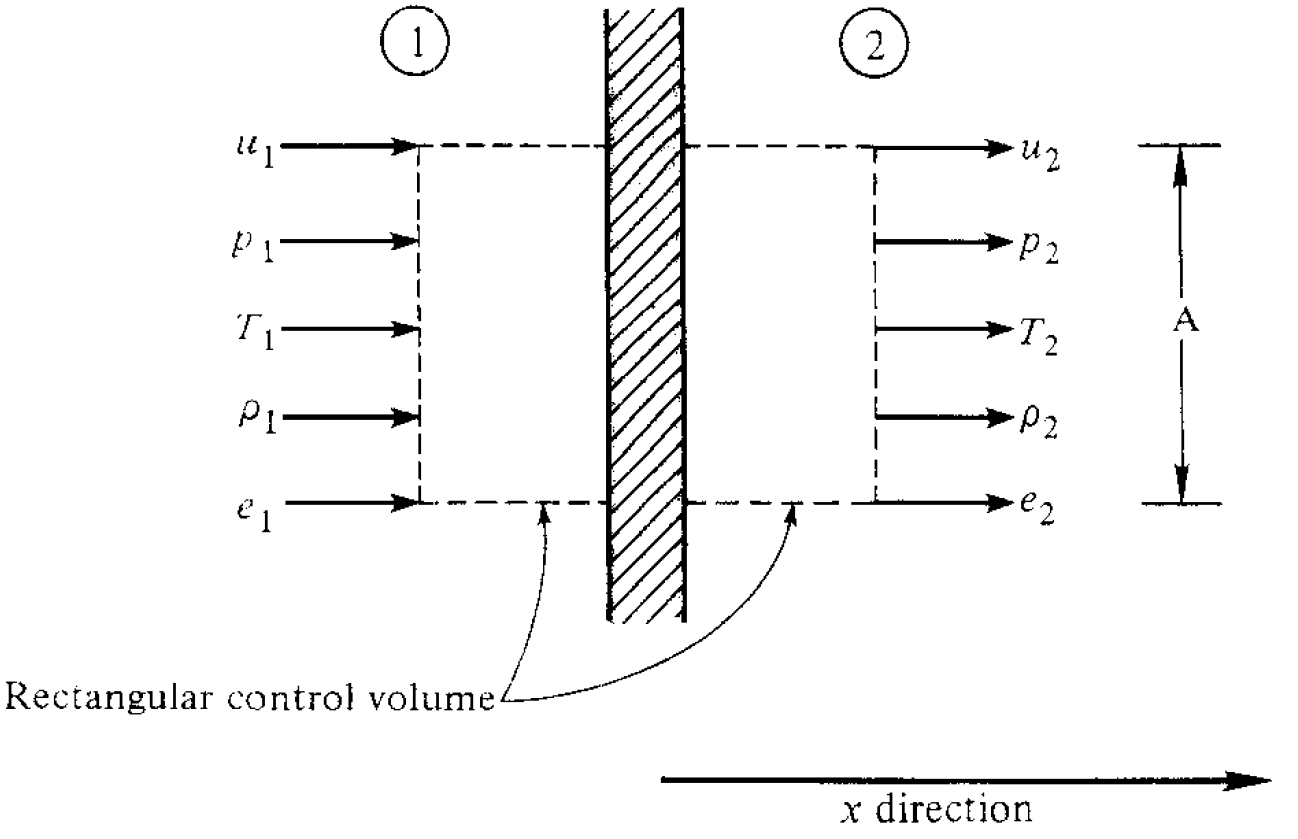
\includegraphics[scale=0.5]{images/problem3_diagram.png}
\end{figure}

In our one-dimensional, steady analyses, we will make the following assumptions about our flow:

\begin{enumerate}[label = (\roman*)]

    \item One-dimensional in the $x$ direction
    \item Steady
    \item Uniform velocity, pressure, temperature, density, enthalpy, and energy at each of the two control surfaces
    \item Flow is perpendicular to control surfaces 1 and 2
    \item \(A_1 = A_2\)
    \item No body forces present
    \item No friction/shear (i.e., there are no solid boundaries around)
    \item No work is done
    \item The pressures acting on the control volume in the $y$ and $z$ directions apply no net force

\end{enumerate}

\begin{enumerate}[label = (\alph*)]

    \item 
        Under these assumptions for one-dimensional, steady flow, show that the integral form of the continuity equation simplifies to
        \[
            \rho_1 u_1 = \rho_2 u_2 \, .  
        \]
        You must start with the full integral form and indicate which assumption(s) allowed you to make each simplification.
   
    \item 
        Can the schematic above and assumption (iii) really be valid for compressible flow?
        Explain your reasoning.

    \item 
        What would the result be if we assumed ``quasi-one-dimensional flow''?
        Note, the only difference between one-dimensional flow and quasi-one-dimensional flow is that assumption (v) is no longer valid for quasi-one-dimensional flow.

    \item
        Under the assumptions for one-dimensional, steadu flow, show that the integral form of the $x$-momentum equation simplifies to
        \[
            p_1 + \rho_1 u_1^2 = p_1 + \rho_2 u_2^2 \, .
        \]
        You must start with the full integral form and indicate which assumption(s) allowed you to make each simplification.

    \item
        What would the $y$ and $z$-momentum equations simplify to?

    \item
        Is assumption (vii) ever a good assumption for compressible flows?
        If you think it is, give a realistic application/example of when it is.
        If you don't think it is, explain why not.

    \item
        Under the assumptions for one-dimensional, steadu flow, show that the integral form of the energy equation simplifies to
        \[
            h_1 + \frac{u_1^2}{2} + q = h_2 + \frac{u_2^2}{2}  
        \]
        You must start with the full integral form and indicate which assumption(s) allowed you to make each simplification.
        $q$ is the mass-specific heat.
        
\end{enumerate}


\end{document}